%% SmartLocker, ACM single-column (manuscript) version for ICIIT 2027 (ACM ICPS), condensed to 10 pages.
%% Condensed from ../smartlocker-10p.tex, which stays the full reference copy: the text is shortened, every number
%% is taken from it, and its Figs. 2, 3, 4, 6, 7 and Tables II, V, VIII, IX are left out (their key facts are in the text).
%% Build: tectonic -X compile smartlocker-acm-10p.tex  (uses acmart.cls v1.90a and ACM-Reference-Format.bst
%% from the ICIIT template package, copied into this folder)
\documentclass[manuscript,screen]{acmart}

\usepackage{booktabs}
\usepackage{array}
\usepackage{textcomp}
\usepackage{adjustbox}
\usepackage{tikz}
\usetikzlibrary{arrows.meta,positioning,fit,shapes.geometric,calc,backgrounds}
\graphicspath{{../}}   % images/ is shared with the IEEE version in docs/paper
\newcommand{\revisioncommit}{fd05eb9}
\setlength{\emergencystretch}{2em}   % long \texttt names in the narrow two-column layout
\raggedbottom                        % no stretched gaps above headings when a float ends a column early
% Pastel fills, borders and TikZ styles shared with the IEEE version
\definecolor{slBlue}{HTML}{DCEBFA}   % light blue: clients, entry points
\definecolor{slMint}{HTML}{DDF3E3}   % mint green: server, processing
\definecolor{slYellow}{HTML}{FFF3C4} % pale yellow: decisions, services
\definecolor{slPeach}{HTML}{FFE2C8}  % peach: hardware outputs, data access
\definecolor{slCoral}{HTML}{FFD9D6}  % light coral/pink: alerts, outcomes
\definecolor{slSky}{HTML}{E9F6FB}    % very light cyan: group backgrounds
% Dark borders (one per fill) and ink
\definecolor{slBlueD}{HTML}{1F4E79}
\definecolor{slMintD}{HTML}{1E6B3A}
\definecolor{slYellowD}{HTML}{7A5B00}
\definecolor{slPeachD}{HTML}{8A4513}
\definecolor{slCoralD}{HTML}{9B2226}
\definecolor{slInk}{HTML}{0F2338}    % arrows and lines (dark navy)

\tikzset{
  slbox/.style={draw=slBlueD, fill=slBlue, rounded corners=3pt, line width=0.7pt, align=center,
                font=\small, text=black, inner xsep=5pt, inner ysep=4pt, minimum height=0.8cm},
  slblue/.style={slbox},
  slmint/.style={slbox, draw=slMintD, fill=slMint},
  slyellow/.style={slbox, draw=slYellowD, fill=slYellow},
  slpeach/.style={slbox, draw=slPeachD, fill=slPeach},
  slcoral/.style={slbox, draw=slCoralD, fill=slCoral},
  sldec/.style={draw=slYellowD, fill=slYellow, diamond, aspect=2.1, line width=0.7pt, align=center,
                font=\small, text=black, inner sep=1pt},
  slterm/.style={slbox, draw=slCoralD, fill=slCoral, line width=1.0pt},
  slok/.style={slbox, draw=slMintD, fill=slMint, line width=1.0pt},
  slarr/.style={draw=slInk, line width=0.8pt, -{Latex[length=2.4mm, width=1.7mm]}},
  sldbl/.style={draw=slInk, line width=0.8pt, {Latex[length=2.4mm, width=1.7mm]}-{Latex[length=2.4mm, width=1.7mm]}},
  slret/.style={slarr, dashed},
  sllbl/.style={font=\small, text=black, inner sep=2pt},
  slbus/.style={font=\footnotesize, text=slInk, fill=white, inner sep=1.5pt},
  slgroup/.style={draw=slMintD, dashed, rounded corners=5pt, line width=0.7pt},
  slgrouplbl/.style={font=\small\bfseries, text=slMintD, inner sep=2pt},
}
\newcommand{\slsub}[1]{\\[-1pt]{\footnotesize #1}}
\tikzset{every picture/.style={line width=0.6pt}}

%% Rights and conference data: the rights block is filled in from the ACM rights form at camera-ready time.
\setcopyright{none}
\copyrightyear{2027}
\acmYear{2027}
\acmConference[ICIIT 2027]{2027 12th International Conference on Intelligent Information Technology}{March 04--07,
  2027}{Ho Chi Minh City, Vietnam}
\acmBooktitle{2027 12th International Conference on Intelligent Information Technology (ICIIT 2027), March 04--07,
  2027, Ho Chi Minh City, Vietnam}
\acmDOI{}
\acmISBN{}
\renewcommand\footnotetextcopyrightpermission[1]{}   % review copy only: delete this line at camera-ready

\begin{document}

\title{Smart Locker with Anomalous Access Detection Based on IoT Device Telemetry}

\author{Duc Hoang Nguyen}
\authornote{Corresponding author.}
\orcid{0009-0006-9780-8146}
\email{duchoang.nguyen103@gmail.com}
\affiliation{%
  \institution{FPT University}
  \city{Ho Chi Minh City}
  \country{Vietnam}}

\author{Viet Tien Nguyen}
\email{tiennguyen100306@gmail.com}
\affiliation{%
  \institution{FPT University}
  \city{Ho Chi Minh City}
  \country{Vietnam}}

\author{Huy Hoang Nguyen}
\email{huyhoang.ct06@gmail.com}
\affiliation{%
  \institution{FPT University}
  \city{Ho Chi Minh City}
  \country{Vietnam}}

\author{Thanh Cao Nguyen}
\email{thanhcao19112006@gmail.com}
\affiliation{%
  \institution{FPT University}
  \city{Ho Chi Minh City}
  \country{Vietnam}}

\author{Thu Le}
\email{thulvm@fpt.edu.vn}
\affiliation{%
  \institution{FPT University}
  \city{Ho Chi Minh City}
  \country{Vietnam}}

\author{Trong Khanh Kieu}
\email{khanhkt@fpt.edu.vn}
\affiliation{%
  \institution{FPT University}
  \city{Ho Chi Minh City}
  \country{Vietnam}}

%% The manuscript style prints e-mails only for journals; \thanks prints them as a footnote on page 1.
\thanks{Authors' e-mails: D. H. Nguyen (corresponding author), duchoang.nguyen103@gmail.com; V. T. Nguyen,
  tiennguyen100306@gmail.com; H. H. Nguyen, huyhoang.ct06@gmail.com; T. C. Nguyen, thanhcao19112006@gmail.com;
  T. Le, thulvm@fpt.edu.vn; T. K. Kieu, khanhkt@fpt.edu.vn.}

\renewcommand{\shortauthors}{D. H. Nguyen et al.}

\begin{abstract}
Shared lockers on university campuses are still opened with mechanical keys or paper codes, cannot be reserved,
and give staff no view of forced doors, lost keys or forgotten items; once networked, their unlock signal can also be
forged or replayed. This paper presents SmartLocker, a locker rental system in which users reserve a slot on a web map,
pay from a prepaid wallet and open it with a personal identification number (PIN), a radio-frequency identification
(RFID) card, a fingerprint or a phone page. The ESP32 box takes no access decision: it forwards every credential to the
server, which replies \texttt{UNLOCK} or \texttt{DENY}. Abnormal access is detected mainly by a priority-ordered rule
engine that uses device telemetry and server context to recognize sensor faults, spoofed remote opens, lost cards,
forced opening, wrong-user access, items left behind and overdue storage. A machine-learning risk score is kept only as
a secondary signal and raises an alert for sessions that no rule explains. On synthetic labeled sessions, the best of
four Weka classifiers made almost all of its errors between wrong-user and normal sessions, which share the same
telemetry by construction; identity is therefore checked by rule, and the score should be trusted only once real
sessions are available. All automated tests and the replayed detection scenarios passed, and in local tests on one laptop the server-side
processing of every timed device request took under 40~ms. In a pre-deployment simulation sent through the live device API, a multi-sensor rule prototype outperformed a
partial-parity rule comparator (macro-F1 0.780 against 0.658) but missed most tamper sessions and stayed below learned
classifiers; because the simulated distributions are assumed, these results do not predict field performance.
\end{abstract}

\begin{CCSXML}
<ccs2012>
 <concept>
  <concept_id>10002978.10002997.10002999</concept_id>
  <concept_desc>Security and privacy~Intrusion detection systems</concept_desc>
  <concept_significance>500</concept_significance>
 </concept>
 <concept>
  <concept_id>10010520.10010553</concept_id>
  <concept_desc>Computer systems organization~Embedded and cyber-physical systems</concept_desc>
  <concept_significance>300</concept_significance>
 </concept>
 <concept>
  <concept_id>10010147.10010257</concept_id>
  <concept_desc>Computing methodologies~Machine learning</concept_desc>
  <concept_significance>100</concept_significance>
 </concept>
</ccs2012>
\end{CCSXML}

\ccsdesc[500]{Security and privacy~Intrusion detection systems}
\ccsdesc[300]{Computer systems organization~Embedded and cyber-physical systems}
\ccsdesc[100]{Computing methodologies~Machine learning}

\keywords{Smart locker, Internet of Things, ESP32, RFID, anomaly detection, rule engine, machine learning, Weka}

\maketitle

\section{Introduction}

Self-service lockers are now common for parcel delivery \cite{iwan2016parcel} and for short-term storage in campuses,
canteens, gyms and libraries, but campus lockers remain mechanical: a key or paper code opens the door, a slot cannot be
booked in advance, and a forced door, a lost key used by someone else or items left for days are noticed only when
reported.
Connecting lockers through the Internet of Things (IoT) \cite{alfuqaha2015iot} makes slot states visible to a server,
but a box can then be impersonated, an unlock message forged or replayed, and sensor readings manipulated
\cite{sicari2015security,roman2013features}.

SmartLocker addresses both the rental service and these threats for a shared campus locker. The box is a thin,
authenticated client and the server takes every decision, since only the server holds the full booking context. The
contributions are listed in Table~\ref{tab:contrib}; the priority-ordered rule tier is the main contribution, whereas
the machine-learning risk score serves as a secondary signal because it is trained on synthetic data only.

\begin{table}[htbp]
\centering
\footnotesize
\caption{Contributions of This Work and Where They Are Shown.}
\label{tab:contrib}
\begin{adjustbox}{max width=\textwidth}
\begin{tabular}{c p{11.9cm} p{2.7cm}}
\toprule
No. & Contribution & Where it is shown \\
\midrule
1 & A locker rental system with map reservation, prepaid wallet, four opening methods (PIN, RFID card, fingerprint and
    phone) and an ESP32 box that forwards every credential with its own device API key; all money and time rules run in SQL transactions. & Sections~\ref{sec:design} and~\ref{sec:impl} \\
2 & A priority-ordered rule engine over telemetry and server context that labels sensor faults, spoofed remote opens,
    lost cards, forced opening, wrong-user access, items left behind and overdue storage, with a hash-chained audit log and a secondary ML risk score. & Section~\ref{sec:detector} \\
3 & An evaluation with automated tests, replayed scenarios and response times, a classifier comparison showing that
    telemetry alone cannot separate wrong-user from normal access, and a simulated multi-sensor study with paired
    statistics, learned baselines, an ablation and a sensitivity analysis. & Section~\ref{sec:ml} \\
\bottomrule
\end{tabular}
\end{adjustbox}
\end{table}

\section{Related Work}

\textit{Smart and parcel lockers.} Research on parcel lockers has concentrated on last-mile logistics, where lockers
reduce failed deliveries and courier trips \cite{iwan2016parcel}, rather than on access security: a recent systematic
review finds only one sustainability study on safety and security \cite{zhang2025parcel}, and users rank a dedicated
application, a matching box size and the station location among the most important attributes
\cite{ciesla2023parcel}. An RFID-based IoT locker \cite{rfidiot2023locker} identifies the user with an identity card
and uses Wi-Fi to monitor the locker, log accesses and watch for unauthorized use; SmartLocker instead checks every
credential in transactional server procedures and combines context rules with telemetry scoring over a hash-chained
audit log.

\textit{Security of IoT devices and credentials.} IoT entities face denial of service, physical damage, eavesdropping,
node capture and loss of control \cite{roman2013features}, and need authentication, access control and trust that
traditional countermeasures cannot provide directly \cite{sicari2015security}; RFID credentials are exposed to cloning,
replay and relay attacks \cite{mitrokotsa2010rfid}. SmartLocker therefore keeps every access decision on the server and
identifies each box with a secret key stored only as a hash.

\textit{Anomaly detection.} Anomaly detection techniques are classification-based (including rule-based), nearest-neighbor,
clustering, statistical, information-theoretic or spectral \cite{chandola2009anomaly}; in IoT, learned detectors
dominate and scarce labeled data favor unsupervised over fully supervised ones \cite{demedeiros2023anomaly}. Like
SmartLocker, Shahin et al. \cite{shahin2025twostage} detect in two tiers: a generative model trained on benign device
traffic flags anomalous IoT traffic and a gradient-boosting classifier labels it, with 99.14\% average end-to-end
accuracy on N-BaIoT. Learned intrusion
detectors are hard to interpret and work best on narrow problems \cite{sommer2010outside}, and 30 machine-learning
papers from top security venues each suffered from at least three of ten common pitfalls (P1 to P10), with sampling bias and data
snooping at least partly present in 90\% and 73\% of them \cite{arp2022dos}. SmartLocker therefore puts explicit rules
in its first tier and uses a Weka model \cite{hall2009weka} only as a supporting score; its audit log is hash-chained as
proposed by Haber and Stornetta \cite{haber1991timestamp}, and passwords are hashed with BCrypt \cite{provos1999bcrypt}.

\section{System Design}\label{sec:design}

\subsection{Architecture, Roles and Data}

SmartLocker has a three-tier architecture (Fig.~\ref{fig:arch}): web browsers, a phone unlock page and the ESP32 locker
box are the clients; a Java~8 Servlet/JSP application following the MVC2 pattern on Apache Tomcat~9 is the
application tier; and a SQL Server database that also implements the business rules as stored procedures is the data
tier. Credentials and telemetry are captured at the box and forwarded to the server, which takes the access decision
and runs the detector; every outcome is stored as a booking change, an alert or an audit entry.

\begin{figure}[htbp]
\centering
\begin{adjustbox}{max width=0.7\textwidth}
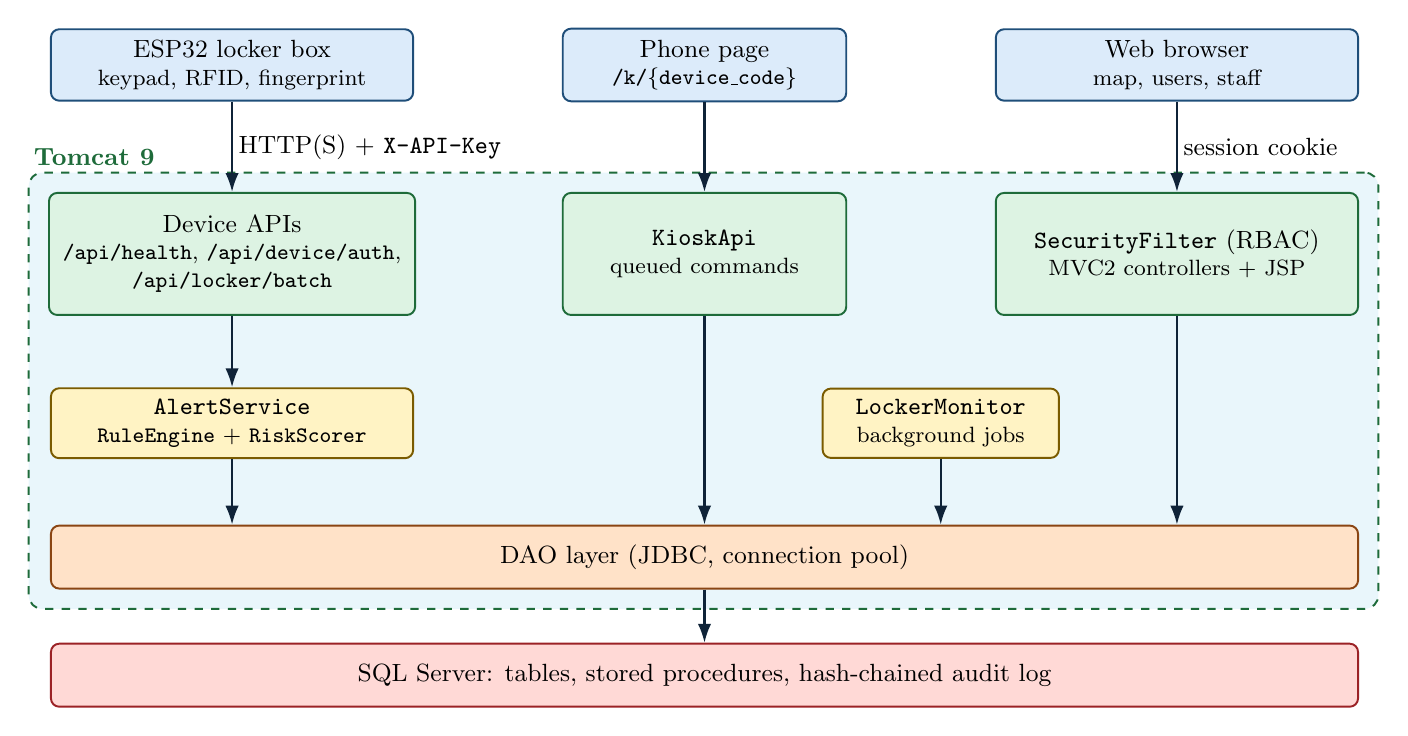
\begin{tikzpicture}
  % clients (top row)
  \node[slblue, minimum width=4.6cm] (esp)   at (2.4,4.3)  {ESP32 locker box\slsub{keypad, RFID, fingerprint}};
  \node[slblue, minimum width=3.6cm] (phone) at (8.4,4.3)  {Phone page\slsub{\texttt{/k/\{device\_code\}}}};
  \node[slblue, minimum width=4.6cm] (web)   at (14.4,4.3) {Web browser\slsub{map, users, staff}};
  % application tier
  \node[slmint, minimum width=4.6cm, minimum height=1.55cm] (devapi) at (2.4,1.9)
       {Device APIs\slsub{\texttt{/api/health}, \texttt{/api/device/auth},}\slsub{\texttt{/api/locker/batch}}};
  \node[slmint, minimum width=3.6cm, minimum height=1.55cm] (kiosk) at (8.4,1.9)
       {\texttt{KioskApi}\slsub{queued commands}};
  \node[slmint, minimum width=4.6cm, minimum height=1.55cm] (ctrl) at (14.4,1.9)
       {\texttt{SecurityFilter} (RBAC)\slsub{MVC2 controllers + JSP}};
  \node[slyellow, minimum width=4.6cm] (svc) at (2.4,-0.25) {\texttt{AlertService}\slsub{\texttt{RuleEngine} + \texttt{RiskScorer}}};
  \node[slyellow, minimum width=3.0cm] (mon) at (11.4,-0.25) {\texttt{LockerMonitor}\slsub{background jobs}};
  \node[slpeach, minimum width=16.6cm] (dao) at (8.4,-1.95) {DAO layer (JDBC, connection pool)};
  % data tier
  \node[slcoral, minimum width=16.6cm] (db) at (8.4,-3.45) {SQL Server: tables, stored procedures, hash-chained audit log};
  % arrows: client to entry point
  \draw[slarr] (esp)   -- node[sllbl, right] {HTTP(S) + \texttt{X-API-Key}} (devapi);
  \draw[slarr] (phone) -- (kiosk);
  \draw[slarr] (web)   -- node[sllbl, right] {session cookie} (ctrl);
  % arrows inside Tomcat
  \draw[slarr] (devapi) -- (svc);
  \draw[slarr] (svc)    -- (svc |- dao.north);
  \draw[slarr] (kiosk)  -- (kiosk |- dao.north);
  \draw[slarr] (mon)    -- (mon |- dao.north);
  \draw[slarr] (ctrl)   -- (ctrl |- dao.north);
  \draw[slarr] (dao)    -- (db);
  \begin{scope}[on background layer]
    \node[slgroup, fill=slSky, fit=(devapi)(kiosk)(ctrl)(svc)(mon)(dao), inner xsep=7pt, inner ysep=7pt,
          label={[slgrouplbl, anchor=south west]north west:Tomcat 9}] (tc) {};
  \end{scope}
\end{tikzpicture}
\end{adjustbox}
\caption{Three-tier architecture of SmartLocker, in which the ESP32 box, the phone page and the web browser reach the
Tomcat application through separate entry points and every outcome is stored in SQL Server.}
\label{fig:arch}
\Description{Block diagram with three clients on top (ESP32 locker box, phone page, web browser), each reaching its own entry point inside Tomcat (device APIs, KioskApi, SecurityFilter with MVC2 controllers), service boxes AlertService and LockerMonitor below, a DAO layer, and SQL Server at the bottom.}
\end{figure}

Role-based access control defines five roles (\texttt{END\_USER}, \texttt{OPERATOR}, \texttt{TECHNICIAN},
\texttt{AUDITOR} and \texttt{ADMIN}); visitors may only browse the map, and all staff actions are recorded in the audit
log. An \emph{area} is a pin on the map, a \emph{bank} is a column of lockers controlled by one device, and a
\emph{slot} is a 20, 40 or 60~cm cube. Filtered unique indexes reject a second open booking for the same slot or user, a
database trigger keeps access sessions append-only, and wallet deductions run inside transactions with exclusive row
locks.

\subsection{Hardware}

The box is built around an ESP32 development board running firmware 4.3: a 4$\times$4 keypad reads PINs, a PN532 NFC
reader reads RFID cards, an AS608 optical sensor reads fingerprints, a 16$\times$2 I$^2$C LCD displays messages, two
servos drive the bolt and the door, and an SRF05 ultrasonic sensor detects a person in front of the box; the door is
locked 20~s after the person has left, or at the latest 120~s after opening. No door switch, load cell or accelerometer is
fitted and the firmware does not upload access sessions, so door time, weight and inertial readings exist only in the
simulator of Section~\ref{sec:sim_eval}, and no physical validation of door, load or tamper sensing is claimed.

\subsection{Device Protocol}

Each box holds a secret API key; the database stores only its SHA-256 hash, and the server derives the device identity
from the key, never from the request body. \texttt{POST /api/health} sends a heartbeat every 3~s and returns pending
commands and blocked card UIDs; \texttt{POST /api/device/auth} submits a PIN, card UID or finger slot and receives
\texttt{UNLOCK}, \texttt{DENY}, \texttt{CHOOSE} (open the slot or check out) or \texttt{CONFIRM\_EMAIL}; and
\texttt{POST /api/locker/batch} uploads
access sessions with a sequence number, so that a resent session is stored only once. When e-mail is enabled, a card
scan unlocks only after the owner confirms through a single-use link, stored only as a hash, or on the map, and a card
at the wrong box is refused with \texttt{WRONG\_PLACE}. An opening at the box is answered at once, whereas a remote or
phone open arrives with the next heartbeat and returns as a session carrying the command id.

\subsection{Booking Lifecycle}

A reservation charges the wallet and holds the slot for 15~minutes, and a booking that was never opened ends as a
\texttt{NO\_SHOW}. An opened booking that becomes overdue is never released, since the items are still inside: after
the grace period the slot is locked, each late hour costs 150\% of the hourly rate, and after 48~hours an
\texttt{OVERDUE\_ESCALATED} alert goes to staff.

\section{Anomalous Access Detection}\label{sec:detector}

\subsection{Access Sessions and Context}\label{sec:sessions}

Each physical door event or rejected card scan produces an \emph{access session} with five features: door time (s),
weight change (g), unlock count, whether a valid local credential was accepted, and stay time (min), together with the
opening source, the presented card UID and, for a remote or phone open, the command id. Because telemetry does not
reveal \emph{who} opened the slot, the server first loads the context: card status and owner, booking owner, whether the
remote command was issued and is still unused, allowed stay, valid sensor ranges, calibration validity and the clock
offset between box and server. The features form the vector $\mathbf{x}_s$ scored by the model, whereas the context is
checked by the rules.

\subsection{Tier 1: Priority-Ordered Rule Engine}

The rules of Table~\ref{tab:rules} are evaluated in a fixed order and the first match determines the label, so that
faulty readings are not reported as a break-in and a legitimate remote open is not reported as a forced opening. The
valid ranges (door 0 to 3600~s, weight change $-200$ to 20\,000~g, stay 0 to 10\,080~min) are stored in the database. Rule 2'
is the negative branch of rule 2; column Tests counts the 13 of the 14 rule-engine unit tests that end in a label, and
S marks rules also reached by a replayed scenario (Section~\ref{sec:functional}).

\begin{table}[htbp]
\centering
\footnotesize
\caption{Detection Rules in Priority Order.}
\label{tab:rules}
\begin{adjustbox}{max width=\textwidth}
\begin{tabular}{c l p{8.1cm} l c}
\toprule
\# & Label & Condition & Action & Tests \\
\midrule
1 & SENSOR\_FAULT & door time, weight change or stay time outside valid range; door open longer than stay; box clock over 300~s ahead; weight calibration expired & Alert, ticket, no ML & 3, S \\[2pt]
2 & STAFF\_OPEN & remote or phone open with a valid, unused command for this slot, issued at most 30~min before the session (box clock up to 60~s behind tolerated) & Command done, no alert & 2, S \\[2pt]
2' & SUSPECTED\_SPOOF & remote or phone open without a valid, unused command & Alert & 1, S \\[2pt]
3 & LOST\_CARD\_USED & the presented card is not active (reported lost or blocked) & Alert & 1, S \\[2pt]
4 & FORCED\_OPEN & the door opened locally without an accepted PIN, active card or fingerprint & Alert & 1 \\[2pt]
5 & WRONG\_USER & an active card whose owner is not the owner of the slot booking & Alert & 1 \\[2pt]
6 & SUSPECTED\_SPOOF & the weight changed by more than 50~g while the door time stayed at 0~s (unreported open) & Alert & 1 \\[2pt]
7 & ITEM\_LEFT & the weight change is above $+50$~g (read as items left after pick-up) & Alert & 1 \\[2pt]
8 & OVERDUE & stay time longer than the plan allows & Alert & 1 \\[2pt]
9 & NORMAL & no rule matched & Tier 2 & 1 \\
\bottomrule
\end{tabular}
\end{adjustbox}
\end{table}

\subsection{Tier 2: Machine-Learning Risk Score}

Let $\mathbf{x}_s = (d, w, u, v, t)$ denote the five features of a session $s$. A classifier trained offline on labeled
sessions estimates the probability that $s$ is normal, and the \emph{risk score} is
\begin{equation}
r(s) = 1 - P\left(y = \text{NORMAL} \mid \mathbf{x}_s\right).
\label{eq:risk}
\end{equation}
The deployed model is the six-class classifier with the highest weighted F1, currently IBk ($k=5$). With $\ell(s)$ the
first label of Table~\ref{tab:rules} that matches $s$ and $\mathcal{L}_0 = \{\text{NORMAL}, \text{STAFF\_OPEN}\}$ the
labels without an alert, the alert for $s$ is
\begin{equation}
A(s) =
\begin{cases}
\ell(s), & \ell(s) \notin \mathcal{L}_0,\\
\text{ML\_ANOMALY}, & \ell(s) = \text{NORMAL} \text{ and } r(s) \geq \tau,\\
\text{none}, & \text{otherwise},
\end{cases}
\label{eq:alert}
\end{equation}
with $\tau = 0.80$, which requires at least four of the five nearest neighbors in IBk to belong to abnormal classes.
When a rule matches, $r(s)$ is stored with its alert as evidence; it is never computed for SENSOR\_FAULT or
STAFF\_OPEN. A STAFF\_OPEN marks its command as done through a conditional update, so of two sessions carrying the same
command only one is a staff open and the other becomes SUSPECTED\_SPOOF, and a SENSOR\_FAULT takes the slot out of
service and opens a maintenance ticket (Fig.~\ref{fig:flow}).

\begin{figure}[htbp]
\centering
\begin{adjustbox}{max width=0.7\textwidth}
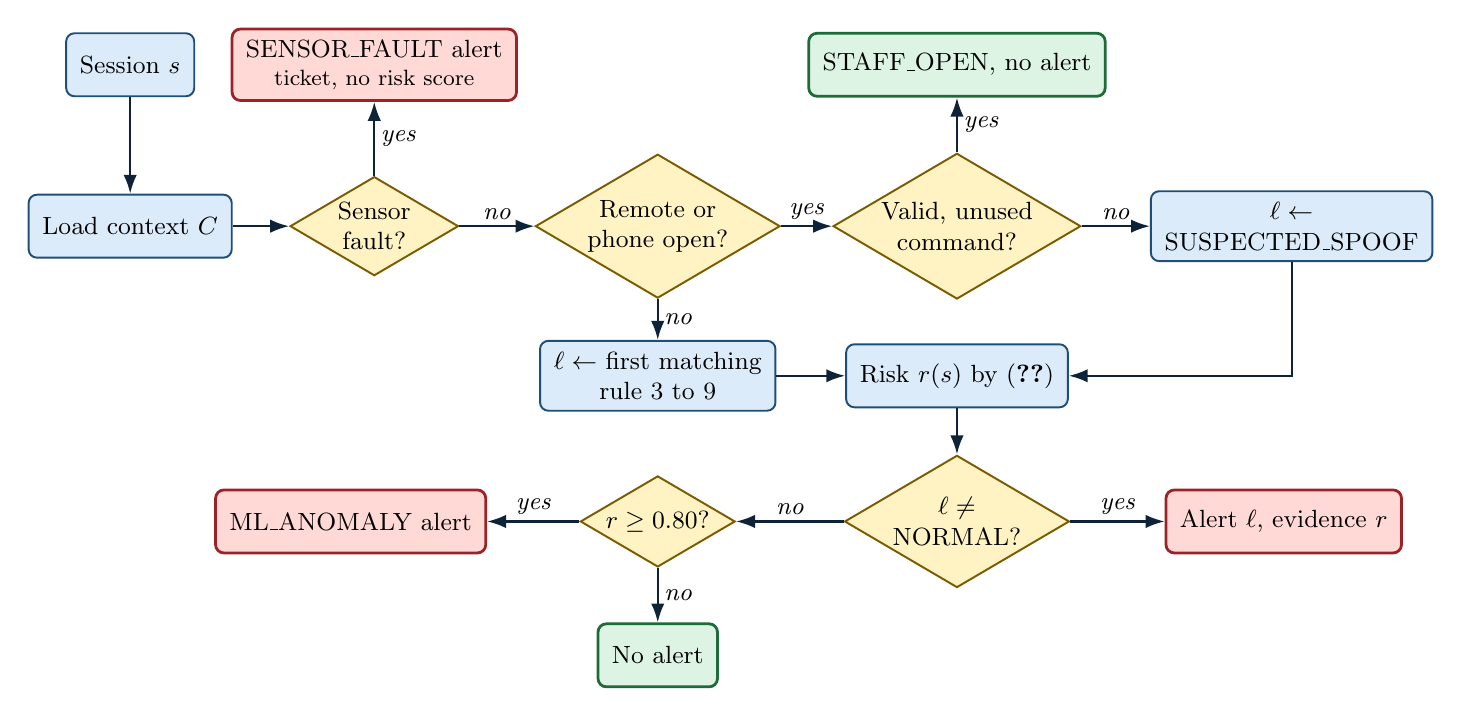
\begin{tikzpicture}[
  proc/.style={slblue},
  dec/.style={sldec, aspect=1.7},
  yes/.style={sllbl, font=\small\itshape},
  no/.style={sllbl, font=\small\itshape}]
  \node[proc]  (in)  at (1.2,2.05)  {Session $s$};
  \node[proc]  (ctx) at (1.2,0)     {Load context $C$};
  \node[dec]   (sf)  at (4.3,0)     {Sensor\\fault?};
  \node[dec]   (rem) at (7.9,0)     {Remote or\\phone open?};
  \node[dec]   (cmd) at (11.7,0)    {Valid, unused\\command?};
  \node[proc]  (spf) at (15.95,0)   {$\ell \leftarrow$\\SUSPECTED\_SPOOF};
  \node[slterm] (flt) at (4.3,2.05)  {SENSOR\_FAULT alert\slsub{ticket, no risk score}};
  \node[slok]   (stf) at (11.7,2.05) {STAFF\_OPEN, no alert};
  \node[proc]  (rul) at (7.9,-1.9)  {$\ell \leftarrow$ first matching\\rule 3 to 9};
  \node[proc]  (rsk) at (11.7,-1.9) {Risk $r(s)$ by (\ref{eq:risk})};
  \node[dec]   (lab) at (11.7,-3.75) {$\ell \neq$\\NORMAL?};
  \node[slterm] (ar) at (15.85,-3.75) {Alert $\ell$, evidence $r$};
  \node[dec]   (thr) at (7.9,-3.75)  {$r \geq 0.80$?};
  \node[slterm] (am) at (4.0,-3.75)  {ML\_ANOMALY alert};
  \node[slok]  (non) at (7.9,-5.45)  {No alert};
  \draw[slarr] (in) -- (ctx);
  \draw[slarr] (ctx) -- (sf);
  \draw[slarr] (sf) -- node[yes, right] {yes} (flt);
  \draw[slarr] (sf) -- node[no, above] {no} (rem);
  \draw[slarr] (rem) -- node[yes, above] {yes} (cmd);
  \draw[slarr] (rem) -- node[no, right] {no} (rul);
  \draw[slarr] (cmd) -- node[yes, right] {yes} (stf);
  \draw[slarr] (cmd) -- node[no, above] {no} (spf);
  \draw[slarr] (rul) -- (rsk);
  \draw[slarr] (spf) |- (rsk);
  \draw[slarr] (rsk) -- (lab);
  \draw[slarr] (lab) -- node[yes, above] {yes} (ar);
  \draw[slarr] (lab) -- node[no, above] {no} (thr);
  \draw[slarr] (thr) -- node[yes, above] {yes} (am);
  \draw[slarr] (thr) -- node[no, right] {no} (non);
\end{tikzpicture}
\end{adjustbox}
\caption{Decision flow of the two-tier detector for one access session: the rules of Table~\ref{tab:rules} run first,
and the risk score raises an ML\_ANOMALY alert only when no rule matched, as in (\ref{eq:alert}); outcome boxes have a
thick border, coral for an alert and mint otherwise.}
\label{fig:flow}
\Description{Flowchart of the two-tier detector: a sensor fault check, the remote-open and command checks, rules 3 to 9, the risk score, and the final choice between a rule alert, an ML_ANOMALY alert and no alert.}
\end{figure}

\subsection{Server-Side Safeguards and Audit Log}\label{sec:safeguards}

Some anomalies need no telemetry: five wrong PINs, cards or fingers within 5~minutes lock the box for 120~s; a job
running every 15~s marks a box silent for 90~s as \texttt{OFFLINE} and raises a \texttt{DEVICE\_OFFLINE} alert; a card
reported lost is pushed to the box in the blocked list of the next heartbeat; and a valid card at the wrong box is
logged as \texttt{WRONG\_PLACE}. Every business action and alert is appended to an audit log whose entries store the
SHA-256 hash of their fields and of the previous entry \cite{haber1991timestamp}. The
last entry is read under an update lock, so concurrent writers cannot fork the chain, and altering, deleting,
inserting or reordering an entry inside the chain breaks the next link; a background job re-verifies the chain every
60~s and raises an integrity alert naming the broken sequence number. Without an external anchor, the chain cannot
reveal removal or addition of the newest entries, nor an administrator who recomputes every hash, so it is
tamper-evident rather than a full time-stamping protocol.

\section{Implementation}\label{sec:impl}

The server is written in Java~8 (about 11\,800 lines including comments and blank lines, in 89 source files) with
22 JSP views and uses Gson, jBCrypt \cite{provos1999bcrypt} and Weka \cite{hall2009weka}. Every rule involving money
or time is a stored procedure that locks the rows it modifies with \texttt{UPDLOCK, HOLDLOCK}, so a slot cannot be
booked twice and an extension cannot be charged twice. Every query that carries user input is a JDBC prepared
statement, user data is escaped in JSP and JavaScript, no script is loaded from a content delivery network, and every
state-modifying request except sign-up and sign-in needs a permitted signed-in user, the PIN of the phone page or a
single-use e-mail token.

\section{Evaluation}\label{sec:ml}

\subsection{Experimental Setup}

\textit{Dataset.} The risk model is trained on 480 rows of the five features and a label, generated by the group's seed
script \texttt{sql/02\_data\_v1.sql} with 80 rows in each of six classes (NORMAL, FORCED\_OPEN, WRONG\_USER, OVERDUE,
ITEM\_LEFT and SUSPECTED\_SPOOF); no public dataset, such as TON\_IoT \cite{moustafa2021toniot}, records the door time,
weight change and card of a locker session. The rows are synthetic, generated from simple class patterns such as no
valid card, a long door time and multiple unlocks for forced opening; wrong-user rows use the same formulas as normal
ones and differ only in the row index, and the rows form a deterministic grid rather than a random sample.

\textit{Protocol.} Random Forest \cite{breiman2001rf}, J48 (C4.5) \cite{quinlan1993c45}, Naive Bayes \cite{john1995nb}
and IBk \cite{aha1991ibl} were compared with Weka defaults, except $k=5$ for IBk, by stratified 10-fold cross-validation
\cite{kohavi1995cv} (seed 42) on the six classes and on a binary NORMAL-versus-ABNORMAL task. All runs used one laptop
(Intel Core i5-11400H, 16~GB RAM, Windows~11; JDK 1.8.0\_202, Weka 3.8.6, Tomcat 9.0.113, SQL Server 2022). All tests and
measurements ran on 17 November 2026 on commit \texttt{\revisioncommit}, to which the code counts also refer; its server,
TestNG and SQL code is unchanged in the final commit. The Weka metrics equal those of a run on 30 October 2026, and the
simulation ran on 16 November 2026 (UTC) on the same code.

\subsection{Classification Results}

IBk achieves the highest weighted F1 on both tasks (Table~\ref{tab:ml} and Fig.~\ref{fig:eval}(a)),
followed by Random Forest, while Naive Bayes is the weakest model in the six-class setting. IBk classifies all
FORCED\_OPEN, OVERDUE and SUSPECTED\_SPOOF sessions and 79 of 80 ITEM\_LEFT sessions correctly; 10 of its 11 errors are
wrong-user sessions labeled normal (7) or the reverse (3; Fig.~\ref{fig:eval}(b)), and Random Forest errs the same way
(17 and 8). A valid card of another person produces the telemetry of a normal visit, and without the 80 WRONG\_USER rows IBk
misclassifies only 1 of 400 sessions (99.75\% accuracy). Wrong-user access is therefore answered exactly by rule~5,
ML alerts are shown to staff as model detections rather than rule matches \cite{sommer2010outside}, and the risk
score should be trusted only after retraining on labeled real sessions.

\begin{table}[tbp]
\centering
\small
\caption{Offline Weka Study on the 480-Row Dataset (Weighted Averages, Stratified 10-Fold Cross-Validation).}
\label{tab:ml}
\begin{adjustbox}{max width=\textwidth}
\begin{tabular}{l c c c c c c}
\toprule
 & \multicolumn{4}{c}{Six classes / Multi-class} & \multicolumn{2}{c}{Binary / Detection} \\
Model & Accuracy & Precision & Recall & F1 & Accuracy & F1 \\
\midrule
Random Forest & 0.948 & 0.949 & 0.948 & 0.948 & 0.938 & 0.939 \\
J48 (C4.5)    & 0.856 & 0.857 & 0.856 & 0.856 & 0.831 & 0.848 \\
Naive Bayes   & 0.779 & 0.778 & 0.779 & 0.778 & 0.833 & 0.852 \\
IBk ($k=5$)   & 0.977 & 0.978 & 0.977 & 0.977 & 0.975 & 0.975 \\
\bottomrule
\end{tabular}
\end{adjustbox}
\end{table}

\begin{figure}[htbp]
\centering
\begin{adjustbox}{max width=\textwidth}
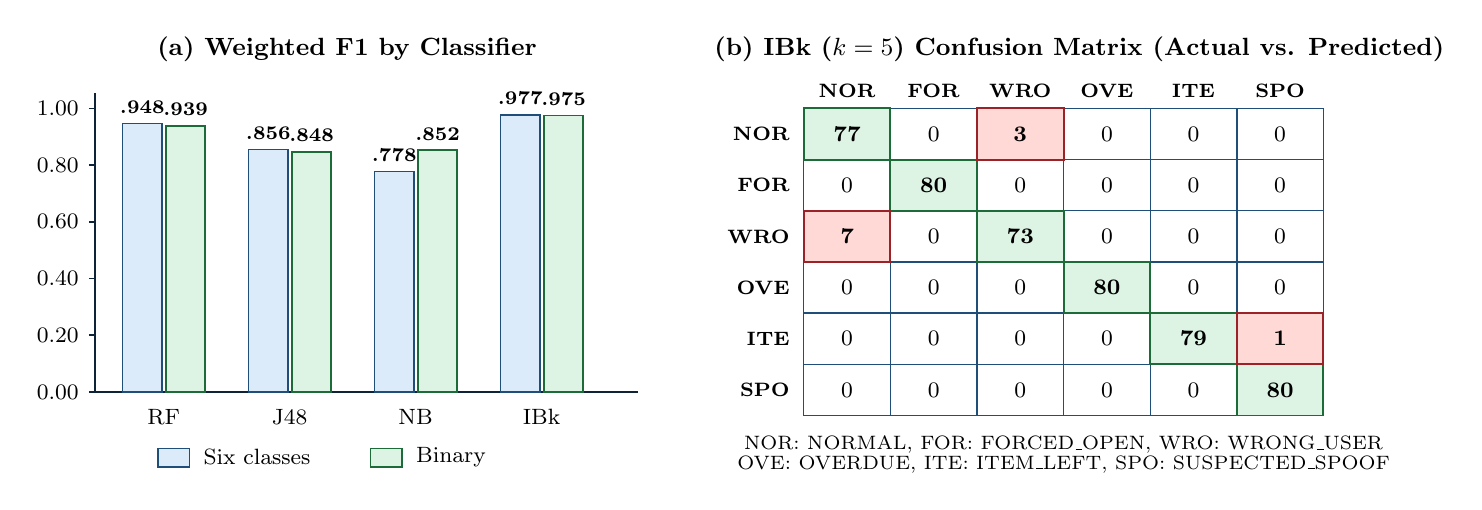
\begin{tikzpicture}
  % Panel (a): Grouped bar chart of Weighted F1 (0.00 to 1.00)
  \node[font=\small\bfseries, text=black] at (4.0, 4.35) {(a) Weighted F1 by Classifier};
  \draw[draw=slInk, line width=0.7pt] (0.8,0) -- (7.7,0);
  \draw[draw=slInk, line width=0.7pt] (0.8,0) -- (0.8,3.8);
  \foreach \y/\lbl in {0.0/0.00, 0.72/0.20, 1.44/0.40, 2.16/0.60, 2.88/0.80, 3.60/1.00} {
    \draw[draw=slInk] (0.72,\y) -- (0.8,\y);
    \node[font=\footnotesize, left] at (0.72,\y) {\lbl};
  }
  % Bars: height = F1 * 3.60
  % RF (Six-class 0.948 -> 3.41, Binary 0.939 -> 3.38)
  \filldraw[draw=slBlueD, fill=slBlue, line width=0.6pt] (1.15,0) rectangle (1.65,3.41);
  \node[font=\scriptsize\bfseries, above] at (1.40,3.41) {.948};
  \filldraw[draw=slMintD, fill=slMint, line width=0.6pt] (1.70,0) rectangle (2.20,3.38);
  \node[font=\scriptsize\bfseries, above] at (1.95,3.38) {.939};
  \node[font=\footnotesize] at (1.67,-0.32) {RF};
  % J48 (Six-class 0.856 -> 3.08, Binary 0.848 -> 3.05)
  \filldraw[draw=slBlueD, fill=slBlue, line width=0.6pt] (2.75,0) rectangle (3.25,3.08);
  \node[font=\scriptsize\bfseries, above] at (3.00,3.08) {.856};
  \filldraw[draw=slMintD, fill=slMint, line width=0.6pt] (3.30,0) rectangle (3.80,3.05);
  \node[font=\scriptsize\bfseries, above] at (3.55,3.05) {.848};
  \node[font=\footnotesize] at (3.27,-0.32) {J48};
  % NB (Six-class 0.778 -> 2.80, Binary 0.852 -> 3.07)
  \filldraw[draw=slBlueD, fill=slBlue, line width=0.6pt] (4.35,0) rectangle (4.85,2.80);
  \node[font=\scriptsize\bfseries, above] at (4.60,2.80) {.778};
  \filldraw[draw=slMintD, fill=slMint, line width=0.6pt] (4.90,0) rectangle (5.40,3.07);
  \node[font=\scriptsize\bfseries, above] at (5.15,3.07) {.852};
  \node[font=\footnotesize] at (4.87,-0.32) {NB};
  % IBk (Six-class 0.977 -> 3.52, Binary 0.975 -> 3.51)
  \filldraw[draw=slBlueD, fill=slBlue, line width=0.6pt] (5.95,0) rectangle (6.45,3.52);
  \node[font=\scriptsize\bfseries, above] at (6.20,3.52) {.977};
  \filldraw[draw=slMintD, fill=slMint, line width=0.6pt] (6.50,0) rectangle (7.00,3.51);
  \node[font=\scriptsize\bfseries, above] at (6.75,3.51) {.975};
  \node[font=\footnotesize] at (6.47,-0.32) {IBk};
  % Legend
  \filldraw[draw=slBlueD, fill=slBlue] (1.6,-0.95) rectangle (2.0,-0.72);
  \node[font=\footnotesize, right] at (2.05,-0.83) {Six classes};
  \filldraw[draw=slMintD, fill=slMint] (4.3,-0.95) rectangle (4.7,-0.72);
  \node[font=\footnotesize, right] at (4.75,-0.83) {Binary};

  % Panel (b): 6x6 Confusion Matrix of IBk (k=5)
  \node[font=\small\bfseries, text=black] at (13.3, 4.35) {(b) IBk ($k=5$) Confusion Matrix (Actual vs. Predicted)};
  \foreach \col/\clbl in {0/NOR, 1/FOR, 2/WRO, 3/OVE, 4/ITE, 5/SPO} {
    \node[font=\scriptsize\bfseries] at ({10.35 + \col*1.1}, 3.82) {\clbl};
  }
  \foreach \row/\rlbl in {0/NOR, 1/FOR, 2/WRO, 3/OVE, 4/ITE, 5/SPO} {
    \node[font=\scriptsize\bfseries, left] at (9.75, {3.275 - \row*0.65}) {\rlbl};
  }
  \foreach \r in {0,...,5} {
    \foreach \c in {0,...,5} {
      \filldraw[draw=slBlueD, fill=white, line width=0.5pt]
        ({9.8 + \c*1.1}, {2.95 - \r*0.65}) rectangle ({10.9 + \c*1.1}, {3.6 - \r*0.65});
      \node[font=\footnotesize] at ({10.35 + \c*1.1}, {3.275 - \r*0.65}) {0};
    }
  }
  \foreach \idx/\val in {0/77, 1/80, 2/73, 3/80, 4/79, 5/80} {
    \filldraw[draw=slMintD, fill=slMint, line width=0.7pt]
      ({9.8 + \idx*1.1}, {2.95 - \idx*0.65}) rectangle ({10.9 + \idx*1.1}, {3.6 - \idx*0.65});
    \node[font=\footnotesize\bfseries] at ({10.35 + \idx*1.1}, {3.275 - \idx*0.65}) {\val};
  }
  \filldraw[draw=slCoralD, fill=slCoral, line width=0.7pt]
    ({9.8 + 2*1.1}, {2.95 - 0*0.65}) rectangle ({10.9 + 2*1.1}, {3.6 - 0*0.65});
  \node[font=\footnotesize\bfseries] at ({10.35 + 2*1.1}, {3.275 - 0*0.65}) {3};
  \filldraw[draw=slCoralD, fill=slCoral, line width=0.7pt]
    ({9.8 + 0*1.1}, {2.95 - 2*0.65}) rectangle ({10.9 + 0*1.1}, {3.6 - 2*0.65});
  \node[font=\footnotesize\bfseries] at ({10.35 + 0*1.1}, {3.275 - 2*0.65}) {7};
  \filldraw[draw=slCoralD, fill=slCoral, line width=0.7pt]
    ({9.8 + 5*1.1}, {2.95 - 4*0.65}) rectangle ({10.9 + 5*1.1}, {3.6 - 4*0.65});
  \node[font=\footnotesize\bfseries] at ({10.35 + 5*1.1}, {3.275 - 4*0.65}) {1};
  \node[font=\scriptsize, text=black, align=center] at (13.1,-0.80)
    {NOR: NORMAL, FOR: FORCED\_OPEN, WRO: WRONG\_USER\\[-1pt]OVE: OVERDUE, ITE: ITEM\_LEFT, SPO: SUSPECTED\_SPOOF};
\end{tikzpicture}
\end{adjustbox}
\caption{Classifier comparison and error distribution on the 480-row dataset, showing weighted F1 scores of the four
models on the six-class and binary tasks (left), and the six-class confusion matrix of IBk with $k=5$ where 10 of the 11
errors fall between NORMAL and WRONG\_USER (right).}
\label{fig:eval}
\Description{Left: grouped bar chart of the weighted F1 of four classifiers on the six-class and binary tasks. Right: six-by-six confusion matrix of IBk in which the errors between NORMAL and WRONG_USER are highlighted.}
\end{figure}

\subsection{Functional Testing}\label{sec:functional}

\textit{Tests.} The TestNG suite contains 83 test methods in 14 classes (47 in memory, 36 against database procedures
and HTTP endpoints), covering among others the rule engine (14 tests), the risk scorer, pricing, the audit hash chain,
the device heartbeat and check-in; in the last run all 83 passed. Nineteen Postman/newman scenarios, from the four
opening methods to lockout, no-show, overdue and escalation, executed 241 requests and 514 assertions without a failure
(2~min 29~s).

\textit{Audit chain.} A read-only export of the audit chain of the simulation database (1\,343 entries) was altered in
seven ways, 20 times each with a fixed seed (20261116). Modifying, deleting, inserting or swapping entries inside the
chain were each detected in 20 of 20 cases, whereas appending at the tail, truncating the tail and a privileged rewrite
that recomputes every hash were each detected in 0 of 20 cases, as expected without an external anchor. With a prototype tool that copies
the chain head to a file outside the database after every ten entries, 20 of 20 rewrites and 18 of 20 truncations were
detected, while appending stayed undetected. These are deterministic tests of single operations, not detection rates.

\textit{Concurrency and detection scenarios.} When 50 users reserved one free slot at the same instant and one user
reserved 20 slots at once, exactly one call won each race and only the two winners were charged. A device simulator
replayed six detection scenarios with the API key of the real box LOCKER-01:
a box that fell silent after six heartbeats was marked \texttt{OFFLINE} with a \texttt{DEVICE\_OFFLINE} alert after
99.5~s (expected 90 to 105~s); a staff remote open became STAFF\_OPEN and its replay SUSPECTED\_SPOOF; a remote session
with an unissued command id became SUSPECTED\_SPOOF; a card reported lost raised LOST\_CARD\_USED and was blocked; a
reservation followed by its PIN gave \texttt{UNLOCK} and \texttt{CHECK\_IN}; and a weight change of $-5000$~g raised
SENSOR\_FAULT and put the slot into maintenance. All six produced the expected label, two only after a fix: the
remote-open rule had no clock tolerance and now accepts a session stamped up to 60~s before its command, and the
check-in scenario now sends the PIN to \texttt{/api/device/auth}, as the real box does.

\subsection{Multi-Sensor Simulation}\label{sec:sim_eval}

Channels the box lacks were exercised by a pre-deployment multi-sensor simulation in Python. A generator first fixes a
latent action and its label and only then draws noisy observations (Table~\ref{tab:sensors}), so no label depends on a
detector; it produced 100 sessions, 20 in each of five categories (normal, unauthorized credential, forced door, load or
tamper, and sensor or network fault), and its version~2, parameters and implementation choices were frozen by hash
before any detector ran. On 16 November 2026 (UTC; run \texttt{RUN\_20261116\_171508\_SEED42\_V2}) a harness sent every
credential and session to the device API of the local stack with the key of a simulated box: every expected
\texttt{UNLOCK} or \texttt{DENY} was returned, all 100 sessions were stored, replayed sequence numbers were rejected,
and 99 matched their expected transport outcome (one injected timeout lasted only 3.27~s, below the 5~s limit). Two
Python detectors then labeled the sessions, and the verdicts stored by the production Java path were read back.
\emph{B0} is a comparator in partial parity with the production rules: it re-implements the range, lost-card,
forced-open and closed-door weight rules and the credential result; \emph{B1-P} is a prototype that adds hand-set
thresholds on ultrasonic distance, vibration, tilt, shock and network latency. When the Java verdicts are mapped to the
five categories, ITEM\_LEFT and ML\_ANOMALY count as errors.

\begin{table}[htbp]
\centering
\footnotesize
\caption{Latent Values of the Simulated Channels (Generator Version~2) and Their Provenance.}
\label{tab:sensors}
\begin{adjustbox}{max width=\textwidth}
\begin{tabular}{l >{\raggedright\arraybackslash}p{9.9cm} >{\raggedright\arraybackslash}p{3.5cm}}
\toprule
Channel & Latent value by class; $\mathrm{LN}(m,s)$: log-normal with median $m$ and log-SD $s$ & Provenance \\
\midrule
Door time (s) & $\mathrm{LN}(8,0.5)$; forced $\mathrm{LN}(6,0.7)$; door fault: stay time $+120$~s & assumed \\
Weight (g) & door opened: 85\% $\pm\mathrm{LN}(150,1.0)$, 15\% $N(0,5^2)$; spoof $\pm\mathrm{LN}(80,0.8)$; other tamper
$N(0,5^2)$; never opened 0; range fault $-350$ or $+24\,000$ & assumed \\
Vibration (g) & $\mathrm{LN}(0.05,0.8)$; drill or pry $\mathrm{LN}(0.30,0.7)$; forced $\mathrm{LN}(0.50,0.7)$ & assumed \\
Shock (g) & $1+\mathrm{LN}(0.3,0.9)$; hammer and forced $1+\mathrm{LN}(3,1.0)$; clipped at 16.0 & assumed; clip: per-axis range \cite{mpu6050} \\
Tilt ($^\circ$) & mounting offset $|U(-2.9,2.9)|$; tilt tamper $\mathrm{LN}(3,0.8)$ & assumed; bound from zero-g offset \textpm50~mg \cite{mpu6050} \\
Ultrasonic (cm) & $U(20,50)$; 0 for a stuck sensor & assumed \\
Stay (min) & $U(1,30)$ in every class & assumed \\
Network (ms) & resampled from 100 measured round trips of \texttt{/api/locker/batch} (2.0 to 39.5); timeout: $+U(2000,
15000)$ & local testbed measurement; delay assumed \\
\bottomrule
\end{tabular}
\end{adjustbox}
\\[2pt]
\parbox{0.92\linewidth}{\footnotesize Unnamed classes and modes use the first (normal) distribution of a row; the noise, drift, outlier and quantization operators of the first generator ($\sigma$ 0.15~s, 3.5~g, 0.015~g, 0.35~g, 0.25$^\circ$, 1.2~cm) apply to every latent value; the 16~g clip applies to the scalar peak although the sensor range is per axis.}
\end{table}

\begin{table}[htbp]
\centering
\small
\caption{Detectors on the 100-Session Simulation (Generator Version~2): Live Seed-42 Run and Five Seeds.}
\label{tab:b0_vs_b1}
\begin{adjustbox}{max width=\textwidth}
\begin{tabular}{l c c c c}
\toprule
Detector & Macro-F1 & Tamper recall & Fault recall & Macro-F1, five seeds \\
\midrule
B0 comparator (Python) & 0.658 & 0.150 & 0.500 & $0.610\pm0.038$ \\
B1-P prototype (Python) & 0.780 & 0.250 & 0.950 & $0.753\pm0.036$ \\
Production Java, rules only & 0.616 & 0.150 & 0.500 & live run only \\
Production Java, rules and risk score & 0.475 & 0.150 & 0.500 & live run only \\
J48, trained on the other seeds & 0.980 & 1.000 & 1.000 & $0.980\pm0.010$ \\
Logistic regression, same split & 1.000 & 1.000 & 1.000 & $0.990\pm0.014$ \\
J48 on credential and network fields & 0.546 & 0.000 & 0.250 & $0.537\pm0.022$ \\
\bottomrule
\end{tabular}
\end{adjustbox}
\\[2pt]
\parbox{0.92\linewidth}{\footnotesize Macro-F1 and recall on seed 42; five seeds (42, 101, 202, 303, 404; latent values, credentials, noise and latency vary): mean $\pm$ sample SD; seeds other than 42 were run offline with the expected credential outcome, which the backend returned for all 100 live sessions.}
\end{table}

B1-P reached a macro-F1 of 0.780 against 0.658 for B0 (Table~\ref{tab:b0_vs_b1}), mostly on faults, whose ultrasonic,
inertial and network symptoms lie outside the inputs of B0, while both miss most tamper sessions (B1-P labels 15 of the
20 as normal). For anomaly versus normal, McNemar's test counts 6 sessions that only B1-P gets right and none that only
B0 gets right (exact $p=0.031$), and a stratified paired bootstrap (10\,000 resamples) gives $\Delta$macro-F1 $=0.122$
with a 95\% interval of $[0.062, 0.190]$. The production rules alone reach 0.616 but flag 11 of the 20 normal
sessions: 8 deposits as ITEM\_LEFT, because rule~7 reads every weight gain above 50~g as items left after pick-up, and
3 pick-ups of 233 to 943~g as SENSOR\_FAULT, because rule~1 checks the weight range against the weight change; with the
risk score, 31 sessions
receive an ML\_ANOMALY alert, which carries no class, so macro-F1 falls to 0.475, whereas the anomaly-versus-normal F1
rises from 0.770 to 0.870, level with B1-P (0.871). J48 trained on the other four seeds with all 12 observable
inputs (sensor, credential, latency and replay fields) reaches 0.980 and is right on 19 sessions where B1-P is wrong, against 2 the other way ($p=2.2\times10^{-4}$); logistic
regression on the same split reaches 1.000 (19 against 0), whereas J48 given only the credential and network fields
reaches 0.546, so the labels do not leak through the context. Retrained without one feature group, J48 gives five-seed
means of 0.777 without door and load and 0.881 without the credential context but at least 0.956 without the network, inertial or
ultrasonic group, so door, load and credential data carry most of the information. Scaling the six class-separating
medians of Table~\ref{tab:sensors} by 0.7 or 1.3, one at a time (12 variants) or all together (2), kept B1-P above B0
by 0.12 to 0.16 and below J48 by 0.21 to 0.26 in all 15 runs including the baseline.

\subsection{Server-Side Response Time}\label{sec:latency}

Only the server processing of the device API was timed: 30 requests per endpoint were sent with curl from the same
laptop after one warm-up request, excluding Wi-Fi, credential reading and servo movement. The median was 7.6~ms for the
heartbeat, 16.0~ms for a PIN at the box and 15.9~ms for a PIN on the phone page, and no request took longer than
38.6~ms; a phone-page open also waits for the next 3~s heartbeat. The fifth wrong PIN started a 120~s lock that also
refused the valid PIN, which was accepted again 120.9~s after the lock started.

\subsection{Threats to Validity and Limitations}\label{sec:limits}

\textit{Internal validity.} Both datasets are synthetic: the Weka rows form a deterministic grid, and almost every
simulation distribution is assumed (Table~\ref{tab:sensors}), so the separability J48 exploits reflects these
assumptions (sampling bias, P1 \cite{arp2022dos}). The second generator was designed by authors who knew the B1-P
thresholds, and three of its parameters (the forced-door vibration median, the shock clip and the timeout delay range)
lie within $\pm$20\% of a B1-P threshold, so data snooping (P3) cannot be ruled out; cells the parameter table left open were set
during implementation and approved by the authors only after the run, so they are not preregistered and may lower
tamper recall. B0 has partial parity and a learned tree outperforms B1-P (inappropriate baseline, P6); latent-action
labels, a frozen generator, learned baselines, an ablation, a sensitivity analysis, five seeds and the scripts mitigate
these risks.

\textit{External validity.} All results come from one laptop and one box with a single servo-locked slot; door switch,
load cell and accelerometer are simulated and no campus trace exists (lab-only evaluation, P9), so the simulation does
not establish field performance. Rules 1 and 7 treat every session as the pick-up of a light item: a
deposit of more than 50~g raises ITEM\_LEFT and a pick-up of more than 200~g raises SENSOR\_FAULT, so both should use
the absolute load and the booking phase once a load cell is fitted. Remaining security
risks include the lack of mutual TLS and CSRF tokens, plain HTTP to
Tomcat, unanchored audit rewrites and cloned cards that work until reported. Seeds 42, 101, 202, 303 and 404, the
bootstrap seed 20261116, code, logs and scripts are available at \url{https://github.com/HoangDuc1003/SmartLocker}.

\section{Conclusion}

SmartLocker leaves every access decision of its ESP32 box to the server and labels each access session with a
priority-ordered rule tier backed by a tamper-evident audit log; every replayed scenario gave the expected label, two
after a fix, and median server processing was 7.6 to 16.0~ms per endpoint. Telemetry alone could not separate wrong-user from normal access, so identity is checked by rule.
In a simulation through the live device API, a multi-sensor rule prototype beat a partial-parity comparator (macro-F1
0.780 against 0.658) but found only 5 of 20 tamper sessions and stayed below a learned tree (0.980) and logistic
regression (1.000). Future work will fit a door switch, load cell and accelerometer, base the weight rules on the
absolute load and the booking phase, collect labeled campus sessions, integrate the external anchor into the server,
and add mutual TLS and CSRF tokens.

\begin{acks}
The authors thank FPT University and the instructors. AI tools (Claude, Anthropic) assisted with English editing,
figures and parts of the simulation and evaluation code; the authors reviewed all such material and take full
responsibility for this paper.
\end{acks}

\bibliographystyle{ACM-Reference-Format}
\bibliography{smartlocker-acm}

\end{document}
